\documentclass[aps,reprint,superscriptaddress,11pt]{revtex4-2}
\usepackage{kotex}
\usepackage[HWP]{dhucs-interword}
\usepackage[dvips]{color}
\usepackage{graphicx}
\usepackage{bm}
\usepackage{amsmath}
\usepackage{tikz}

\begin{document}
\title{응집물질물리실험 예비보고서 \\
\small 실험주제 : STM}

\author{HuiJae-Lee}
\affiliation{Physics Department, Inha University}
\email{hjlee6674@inha.edu}
\date{\today}


\begin{abstract}
 이번 실험에서는 STM(주사 터널링 현미경)의 작동원리와 사용 방법에 대해 알아보고 
 Graphite의 표면을 직접 관찰하며 응용해본다. 또한, STM을 이용한 관찰로 부터 결정구조에 대해
 공부하고 이해하는 것을 목표로 한다.
\end{abstract}

\maketitle

\section[Introduction]{Introduction}
STM의 기원은 Ricard Fyenman의 1959년 강연 "There's Plenty of Room at the Bottom: 
An Invitation to Enter a New Field of Physics"에서 찾을 수 있다. 그는 각각의 
원자를 뚜렷하게 보고 우리가 원하는 방식으로 배열하는 새로운 연구 분야를 
제시했고, 그로부터 20년 후 과학자들은 STM(Scanning Tunneling Microscope)과 
AFM(Atomic Force Microscope)의 개발로 그 목표를 달성하기 시작했다. 
STM은 80년대 초 IBM 연구소 소속 Gerd Binning과 Heinrich Rohrer에 의해 개발되었고 
Binning과 Rohrer는 그 공로로 86년 노벨 물리학상을 수상하였다.
STM은 나노 스케일에서의 과학과 기술을 더욱 높은 수준으로 끌어올렸고 기초 물리학에 대한 
이해 또한 엄청나게 발전시켰다. 그 중에서도 이번 실험에 사용할 STM은 3차원에서 표면 구조를 
직접, 실제로 제공한다.
\section[Experiment]{Experiment}
\subsection{Theory}
\subsubsection{양자 터널링}
STM의 원리를 이해하기 위해서는 양자 터널링 현상에 대해 알아야 한다. 양자 터널링은 양자역학과
고전역학의 뚜렷한 차이점 중 하나로, 입자의 동력학적 거동을 해석하는데 파동함수와 확률을
도입하여 설명한다. 
\begin{figure}[htbp]
  \centering
  \begin{tikzpicture}
    %axis
    \draw[-latex] (-4,0)  -- (4,0) node[shift={(-0.1,-0.3)}] {$x$} ;
    \draw[-latex] (0,-1)  -- (0,3) node[shift={(-0.3,-0.1)}] {$y$} ;
    %coordinate
    \coordinate (A) at (-1.5,0);
		\coordinate (B) at (-1.5,1.6);
		\coordinate (C) at ( 1.5,1.6);
    \coordinate (D) at ( 1.5,0);
    %potential
    \draw[] (A)  -- (B);
    \draw[] (B)  -- (C);
    \draw[] (C)  -- (D);
    %wave function
    \draw[-latex] (-4,1)  -- (-1.5,1) node[left=20,above=5] {\large$\psi_{in}$} ;
    \draw[-latex] (1.5,1) node[right=25,above=5] {\large$\psi_{trans}$}  -- (4,1) ;
    %node
		\node[above=10,right] at (0,1.5) {$V_0$};
		\node[below] at (A) {$-a$};
		\node[below] at (D) {$a$};

  \end{tikzpicture}
  \caption{높이 $V_0$와 두께 $2a$의 퍼텐셜 장벽과 
  왼쪽에서 입사하는 자유 입자 $\psi_{in}$}
  \label{fig:1}
\end{figure}
다음과 같은 퍼텐셜 장벽과 이 장벽에 대해 왼쪽에서 입사하는 자유 입자를 
고려하자(FIG.~\ref{fig:1}). 퍼텐셜 장벽의 너비는 $2a$이고 퍼텐셜의 크기는 $V_0$이다. 
중요한 점은 입사하는 자유 입자가 가진 에너지 $E$가 $V_0$보다 작다는 것이다. 
즉, $E<V_0$이다. 이 때 투과확률 $T$는 다음과 같다.
\begin{align}
  \begin{split}
    T=\frac{1}{1+\left(\frac{k^2+q^2}{2kq}\right)^2\sinh^2qa},\,\,\,\\
    k=\sqrt{\frac{2mE}{\hbar^2}},\,\,\,
    q=\sqrt{\frac{2m(V_0-E)}{\hbar^2}}.
  \end{split}
\end{align}
중요한 사실은 투과확률 $T$가 $0$이 아니라는 것이다. 고전역학적으로 보았을 때 
퍼텐셜 장벽보다 낮은 에너지를 가진 입자는 분명히 장벽을 넘을 수 없고 $a<x$영역에는 입자가
존재할 수 없다. 하지만 양자역학적인 해석에 의하면, 투과확률이 존재한다는 것은 입자가 퍼텐셜
장벽을 넘어 $a<x$영역에 존재할 수 있음을 의미한다. 퍼텐셜 장벽이 굉장히 두꺼워 $1<<a$인 경우,
극한을 취하여 근사하면 투과확률 $T$가 $e^{-2qa}$에 비례하게 된다.
\begin{align}
  T\sim \frac{16k^2q^2}{(k^2+q^2)^2}e^{-2qa}.
\end{align}

\subsubsection{STM}
\begin{figure}[htp]
  \centering
  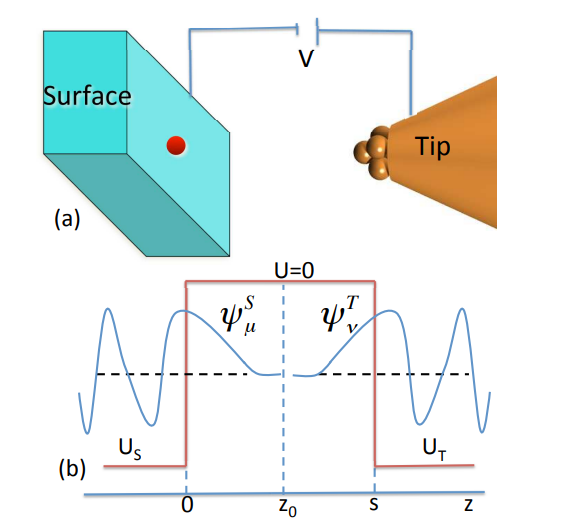
\includegraphics[scale=0.35]{STM.png}
  \caption{(a)는 STM의 대략적인 구조이다. 
  양자 터널링에 의해 전류는 금속 탐침과 물질 사이 진공을 투과하여 흐를 수 있다.
  (b)에서 볼 수 있듯이, 두 전극이 거리를 두고 떨어져 있을 때 두 전극의 파동함수 A와 B는
  진공에서 지수적으로 감소하지만, 가까울 수록 터널링이 많이 일어난다.}
  \label{fig:2}
\end{figure}
STM은 전자의 양자 터널링을 이용해 시료의 표면을 연구할 수 있도록 해준다.
먼저, 시료의 표면을 측정하기 위해 STM에 달린 작은 금속 탐침이 표면에 굉장히 근접한다. 
FIG.~\ref{fig:2}에서 볼 수 있듯이, 이 금속 탐침의 끝은 하나의 원자로 되어있다. 
시료에 전압을 걸어주었을 때 시료와 금속 탐침 사이에는 터널링 전류(tunneling current)가 
측정된다. 시료의 표면에 흐르는 전자가 표면을 탈출하기 위해 STM의 탐침으로 흐르기 위해서는 
원자가 전자를 속박하는 에너지보다 큰 에너지가 필요하다. 이는 위에서 살펴본 퍼텐셜 장벽을 
투과하는 자유 입자의 상황과 유사하다. 원자의 속박 에너지가 퍼텐셜 장벽처럼 작용하는 것이다. 
하지만 투과확률이 $0$보다 크기 때문에 전자는 속박 에너지보다 작은 에너지를 가지더라도 속박 
에너지를 극복하고 STM의 탐침으로 흐를 확률을 가진다. STM은 이렇게 흐르는 전류를 이용하여 
표면에 대한 측정을 시도한다.이 때 금속 탐침이 근접하는 거리는 탐침과 표면 사이의 저항을 측정 
가능할 만큼이다. 시료에 전류가 흘러야 하므로, 도체 시료를 이용한다. 터널링 전류는 탐침과 시료 
사이 터널링 확률(tunneling probability)에 비례하고 이 확률은 거리에 지수적으로 민감하다. 
WKB 근사로부터, 터널링 확률 $P$가 거리 $z$와 다음의 비례관계에 있음을 알 수 있다.
\begin{align}
   P \propto \exp\left(-2\sqrt{\frac{2m\phi}{\hbar^2}z}\right).
\end{align}
$\phi$는 터널링을 위한 유효 장벽의 높이이다. STM은 확률이 거리에 민감하게 반응하는 만큼
정확하게 표면을 측정할 수 있다.


\subsubsection{Graphite}
흑연은 육각형을 배열된 탄소 원자의 층들로 이루어진 탄소의 동소체이다. 층이 쌓이는 배열에는
두가지 형태가 있는데 육각형꼴과 마름모꼴이 있다. 각 층끼리의 화학 결합은 $sp2$ 오비탈 혼성화를
공유하며 C-C거리는 $141.7$~pm이다. 층 사이 약한 결합의 세기가 반데르발스 결합에 비견될 만한
강도를 가진다.
\subsection{Experimental Methods}
\subsubsection{준비}
\begin{itemize}
  \item[1. ] 실험장비를 초기화 한다. 장비의 전원을 켜고 컨트롤러 위 상태 표시등이 모두 켜지는지
  확인한다. Scan Head등과 detected modules등이 깜박이기 시작하고 다른 모든 표시등이 꺼진다.
  프로그램을 시작하면 모든 표시등이 꺼진다. 화면에 “Controller Startup in 
  progress" 문구가 표시되고 module등이 차례로 켜진다. 
  
  초기화가 완료되면 “Starting System"
  메세지가 표시되고 Probe Status등, Scan Head status light등 그리고 detected modules등이 
  켜진다. scan head가 감지되지 않으면 2개의 Scan Head Status등이 깜박인다.
  \item[2. ] STM 탐침을 준비하고 설치한다. 이 때 탐침을 직접 만들어야 하는데 다음의 과정을
  거친다.
  \begin{small}
  \begin{enumerate}
    \item[(1)] wire cutter의 자르는 부분과 Flat nose plier, 핀셋을 에탄올로
    세척한다. 
    \item[(2)] 핀셋으로 기기에서 탐침을 제거한다. 이 탐침이 충분히 길면, 재활용이 가능하다.
    \item[(3)] wire를 Flat nose plier로 잡고 cutter로 wire를 약 4mm 정도 잡아당긴다.
    \item[(4)] cutter에 힘을 주되, wire가 끊어지지 않도록 한다.
    \item[(5)] cutter를 wrie의 방향과 같은 방향으로 잡아당긴다. 좋은 탐침을 얻기 위해서는
    자르지 말고 잡아당겨야 한다(FIG.~\ref{fig:3}).
    \item[(6)] 핀셋으로 새로 만든 탐침을 기기에 설치한다(FIG.~\ref{fig:4}).
      \begin{figure}[htp]
        \centering
        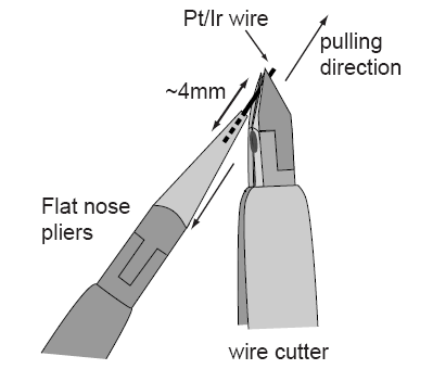
\includegraphics[scale=0.3]{tip.png}
        \caption{탐침을 자르는 방법}
        \label{fig:3}
      \end{figure}
      \begin{figure}[htp]
        \centering
        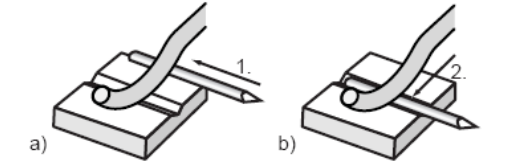
\includegraphics[scale=0.35]{tip2.png}
        \caption{탐침을 설치하는 방법}
        \label{fig:4}
      \end{figure}
  \end{enumerate}
  \end{small}
  \item[3. ] 샘플을 장착한다. 먼저 검은색 플라스틱 부분을 잡고 샘플 홀더를 보관 용기에서 빼낸다.
  이 때 금속 부분은 만져서는 안된다. 이 샘플 홀더를 탐침이 닿지 않도록 하여 기기에 장착한다.
  HOPG(흑연) 샘플을 스카치 테이프로 절단한다. 절단한 샘플을 샘플 홀더와 같이 기기에 장착한다.
  \item[4. ] 샘플과 탐침 사이 거리가 1mm 미만이 되도록 샘플 홀더를 민다(FIG.~\ref{fig:4}). 
  이제 Positioning 창을 열고 magnifier로 탐침과 샘플 사이 거리를 관찰한다. 이 거리는 
  1mm 이내여야 한다. Z-control panel에서 control parameter를 다음과 같이 설정한다: 
  (point=1 nA, P-gain=10000, I-gain=1000, tip voltage=50 mV). 값들을 설정하고 [Approach]를
  누른다. 탐침의 접근이 성공적으로 완료되면 probe status등이 깜박임에서 녹색으로 바뀌고 스캔이
  자동으로 시작된다. 그렇지 않으면, 다시 시도한다.
  \begin{figure}[htp]
    \centering
    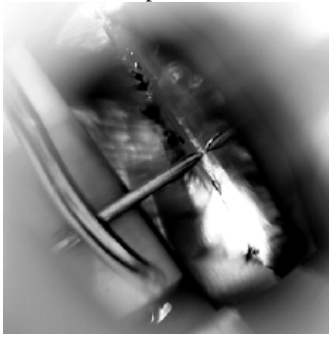
\includegraphics[scale=0.3]{approach.png}
    \caption{탐침과 샘플은 닿지 않아야 한다.}
    \label{fig:4}
  \end{figure}
  \item[5. ] imaging parameter(scan speed, scan direction, tilt, P-gain and I-gain)를 
  조절하고 해상도를 256으로 설정한다. ~500 nm 구간에서 평평한 영역을 찾을 수 있고 원자 해상도
  이미지는 ~4nm 구간이다. 이미지가 원자적 특성을 보여주지 않는다면 스캔 방향을 다르게 하여 다시
  시도한다.
\end{itemize}

\nocite{*}
\bibliography{ref}



%\begin{thebibliography}{9}
%\end{thebibliography}

\vfill
\end{document}